\chapter{Methodology}

\section{Overview}
This chapter outlines the methodology adopted in this study. It includes system modelling, the use of glossary terms such as \gls{mysymbol} and \gls{yoursymbol}, and utilises acronyms such as \gls{phd}. Once the acronym has been introduced, it appears simply as \gls{phd}. For completeness, \acrfull{phd}, \acrshort{phd}, and \glspl{phd} are also demonstrated.

\section{System Model and Notation}
{Enter the material. The symbols and abbreviations defined can be used using the \textbackslash gls command. The defined symbol is \gls{mysymbol} and \gls{yoursymbol}. When the acronym is used for the first time it gives the full form as follows \gls{phd}. Thereafter, it only gives the abbreviation as follows \gls{phd}. The full form, short form and plural of the acronym can be called as follows \acrfull{phd}, \acrshort{phd} and \glspl{phd} respectively.}

\section{Example Figure}
\begin{figure}[!ht]
\centering
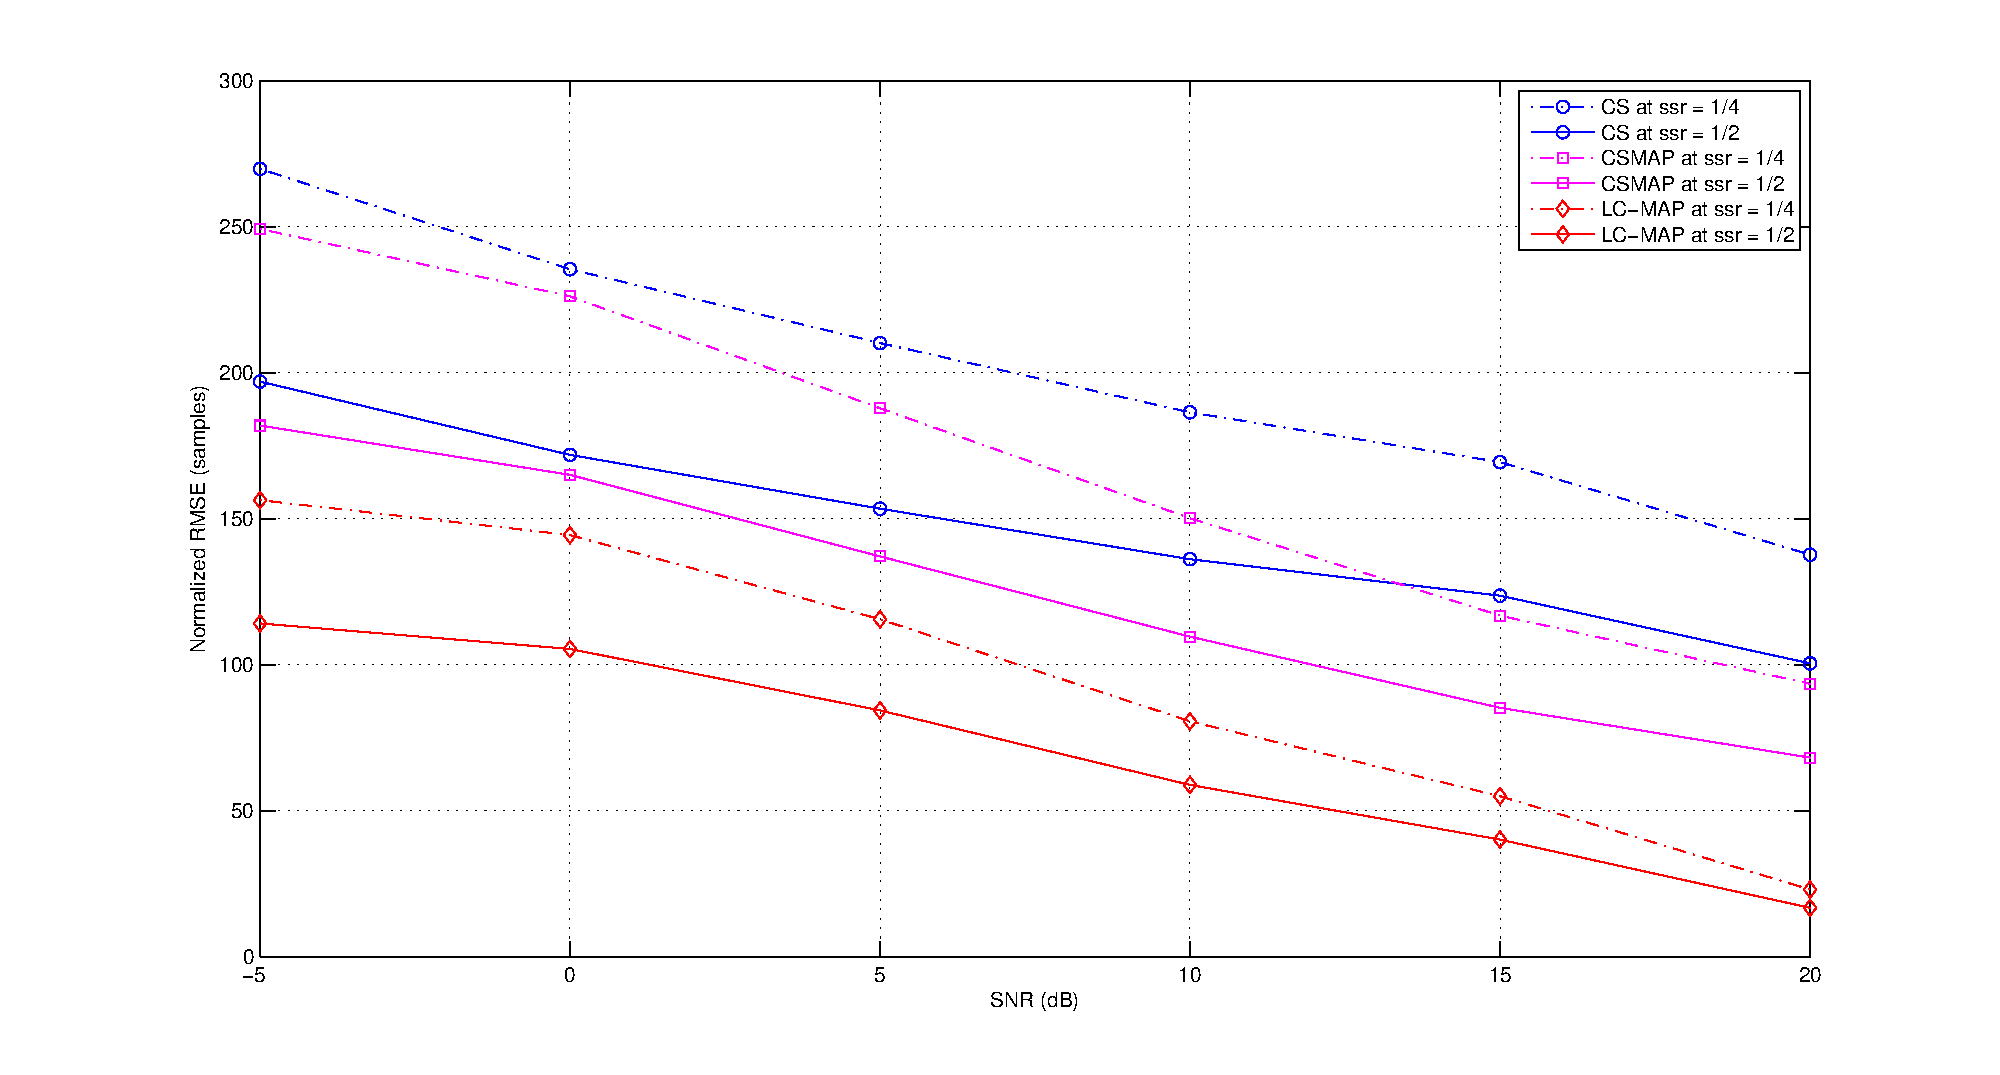
\includegraphics[width=7.5cm, height=5.26cm]{Images/plot.pdf}
\caption{This is a plot to show the results.}
\label{fig:Plot}
\end{figure}

\section{Mathematical Formulation}
{Enter material \cite{Zhang2004}.}

\begin{align}
\label{eq:TimeModel2a}
r(n \delta) &= \sum_{l=0}^{L-1} a_l \, \mathit{g}(\delta - m_l \delta) + \omega(n \delta)
\end{align}

The sub-sampled signal $\mathbf{y}$ at the receiver can be represented in matrix form as:

\begin{equation}
\label{eq:LinModel01}
\mathbf{y} = \mathbf{G} \mathbf{a} + \boldsymbol{\omega}
\end{equation}

where

\begin{equation}
\label{eq:P}
\mathbf{G} = \left[
\begin{matrix}
\mathit{g}(n - m_0) & \cdots & \mathit{g}(n - m_N) \\
\mathit{g}(n + \mu - m_1) & \cdots & \mathit{g}(n + 1 - m_N) \\
\vdots & \ddots & \vdots \\
\mathit{g}(n + \mu - m_M) & \cdots & \mathit{g}(n + \frac{M-1}{\mu} - m_N)
\end{matrix}
\right]
\end{equation}

\section{Additional Section}
{Enter material \cite{Tesi2006}.}

\section{Another Section}
{Enter material \cite{Gezici2009}.}

\subsection{Sub-Section Title}
{Sub-section.}

\subsection{Sub-Sub-Section Title}
{Sub-section \cite{Carbonelli2003}.}

\section{Supplementary Material}
{Enter material \cite{Bajwa2010b}.}

\section{Example Table}

\begin{table}[!ht]
\centering
\begin{tabular}{|c|c|c|c|c|c|c|}
\hline
Itr. No. & $\boldsymbol \Theta_n$ & Size of $\underline{\boldsymbol \alpha}_i$ & \multicolumn{4}{c|}{Residual: $r_i^n = \Vert \mathbf{y} \Vert_{\boldsymbol \Sigma_i}^{2}$} \\ \cline{4-7}
$(n)$ & $(L \times n)$ & $(n \times 1)$ & $i=1$ & $i=2$ & \dots \dots & $i=C$ \\
\hline
1 & $\boldsymbol \Theta_1 = [\boldsymbol \theta_1]$ & $(1 \times 1)$ & $r_1^1$ & $r_2^1$ & \dots \dots & $r_C^1$ \\
\hline
2 & $\boldsymbol \Theta_2 = [\boldsymbol \Theta_1 \boldsymbol \theta_2]$ & $(2 \times 1)$ & $r_1^2$ & $r_2^2$ & \dots \dots & $r_C^2$ \\
\hline
3 & $\boldsymbol \Theta_3 = [\boldsymbol \Theta_2 \boldsymbol \theta_3]$ & $(3 \times 1)$ & $r_1^3$ & $r_2^3$ & \dots \dots & $r_C^3$ \\
\hline
\vdots & \vdots & \vdots & \vdots & \vdots & \dots \dots & \vdots \\
\hline
$L-1$ & $\boldsymbol \Theta_{L-1} = [\boldsymbol \Theta_{L-2} \boldsymbol \theta_{L-1}]$ & $((L-1) \times 1)$ & $r_1^{L-1}$ & $r_2^{L-1}$ & \dots \dots & $r_C^{L-1}$ \\
\hline
$L$ & $\boldsymbol \Theta_L = [\boldsymbol \Theta_{L-1} \boldsymbol \theta_L]$ & $(L \times 1)$ & $r_1^L$ & $r_2^L$ & \dots \dots & $r_C^L$ \\
\hline
\end{tabular}
\caption{This is a Table.}
\label{tab:Table}
\end{table}
